\documentclass[11pt,a4paper]{article}
\usepackage[utf8]{inputenc}
\usepackage{amsmath,amssymb,amsfonts}
\usepackage{graphicx}
\usepackage{geometry}
\usepackage{tikz}
\usepackage{pgfplots}
\usepackage{float}
\usepackage{enumerate}
\usepackage{hyperref}
\usepackage{natbib}
\usepackage{mathtools}
\usepackage{bm}
\usepackage{bbm}

\geometry{margin=1in}
\pgfplotsset{compat=1.17}

\title{The Synthetic Social Graph Theorem: Energy-Based Models for Hyper-Realistic Social Simulations}
\author{Sean McDonald\\
\texttt{x.com/seanmcdonaldxyz}}
\date{Feb 28, 2025}

\begin{document}

\maketitle

\noindent This is an untested, unvetted pre-publication.

\begin{abstract}
This paper presents a novel mathematical framework for modeling complex social dynamics through energy-based models that transcend traditional token-based approaches. The Synthetic Social Graph Theorem integrates tensor representations, wavelet transformations, and synthetic validation mechanisms to create hyper-realistic simulations with unprecedented consistency and fidelity. In this framework, discrete linguistic tokens are replaced with continuous waveforms, social transitions are reconceptualized as energy-gradient flows, and a clockchain mechanism is employed for temporal anchoring. The central formula representing the integrated system is

\begin{align}
X_{t+1} &= (1 - \alpha_t)X_t + \alpha_t \Pi_{S_c}\left(\arg \min_Y \left\{E(Y) = \sum_{i=1}^k w_i \phi_i(Y) + \sum_{i,j} J_{ij} \psi_{ij}(Y_i, Y_j)\right.\right.\nonumber\\
&\quad\left.\left. \prod_{i=1}^m \psi_i(X_t, Y, C_i, H_t) \geq \theta_t\right\} + \eta_t\right)
\end{align}

Recurring behaviors follow ADPRS waveform patterns,
\begin{equation}
f_{\text{ADPRS}}(t) = A e^{-\lambda t} \sum_{k=0}^{\infty} D \text{rect}\left(\frac{t - kP}{D}\right),
\end{equation}

with the entire system organized in a tessellated structure
\begin{equation}
M = \bigcup_{t \in T} \pi^{-1}(t).
\end{equation}

This unified formulation enables the creation of synthetic social simulations with remarkable internal consistency, minimal hallucination, and applicability beyond human social networks to electrical systems, neural networks, and AI-to-AI interactions. By adopting synthesizer-like controls, the framework captures factors beyond linguistic expression, providing a universal approach to modeling complex networked systems.
\end{abstract}

\section{Introduction and Key Theoretical Foundations}

\subsection{Context and Motivation}

The primary innovation of the Synthetic Social Graph Theorem lies not in its individual components but in their integration into a cohesive mathematical framework that transcends traditional approaches to social modeling. Current computational social science largely relies on token-based linguistic models or simplistic agent-based simulations that fail to capture the complex, multi-dimensional nature of human social dynamics. This framework represents an ambitious roadmap for developing systems capable of modeling social phenomena with unprecedented fidelity and coherence.

The limitations of current approaches stem from several key factors:

\begin{itemize}
\item \textbf{Token-Based Constraints}: Language models operate primarily within semantic spaces that cannot adequately represent non-linguistic social patterns.
\item \textbf{Temporal Inconsistency}: Most models lack rigorous temporal anchoring, leading to causality violations and inconsistent behavioral patterns.
\item \textbf{Validation Deficiencies}: Without structured validation mechanisms, hallucinations and inconsistencies proliferate in synthetic social simulations.
\item \textbf{Dimensional Limitations}: Traditional approaches fail to capture the multi-dimensional nature of social identity and interaction.
\end{itemize}

This paper presents a framework that addresses these limitations through an energy-based model approach, leveraging mathematical structures from quantum mechanics, signal processing, and differential geometry to create hyper-valid, hyper-realistic social simulations.

\subsection{Core Theoretical Principles}

The Synthetic Social Graph Theorem rests on four fundamental principles:

\subsubsection{Synthetic Identity Tensors}

\begin{figure}[H]
\centering
% Figure showing synthetic identity tensors and energy states
% Should include: 3D tensor visualization with demographic, behavioral, and psychographic dimensions
% Neural energy states (cognitive, emotional, social) as waveform outputs
% Formula box showing F_i ∈ R^(d1 × d2 × ... × dn) and E(F_i) = Σ w_j φ_j(F_i) + Σ J_ik ψ_ik(F_i, F_k)
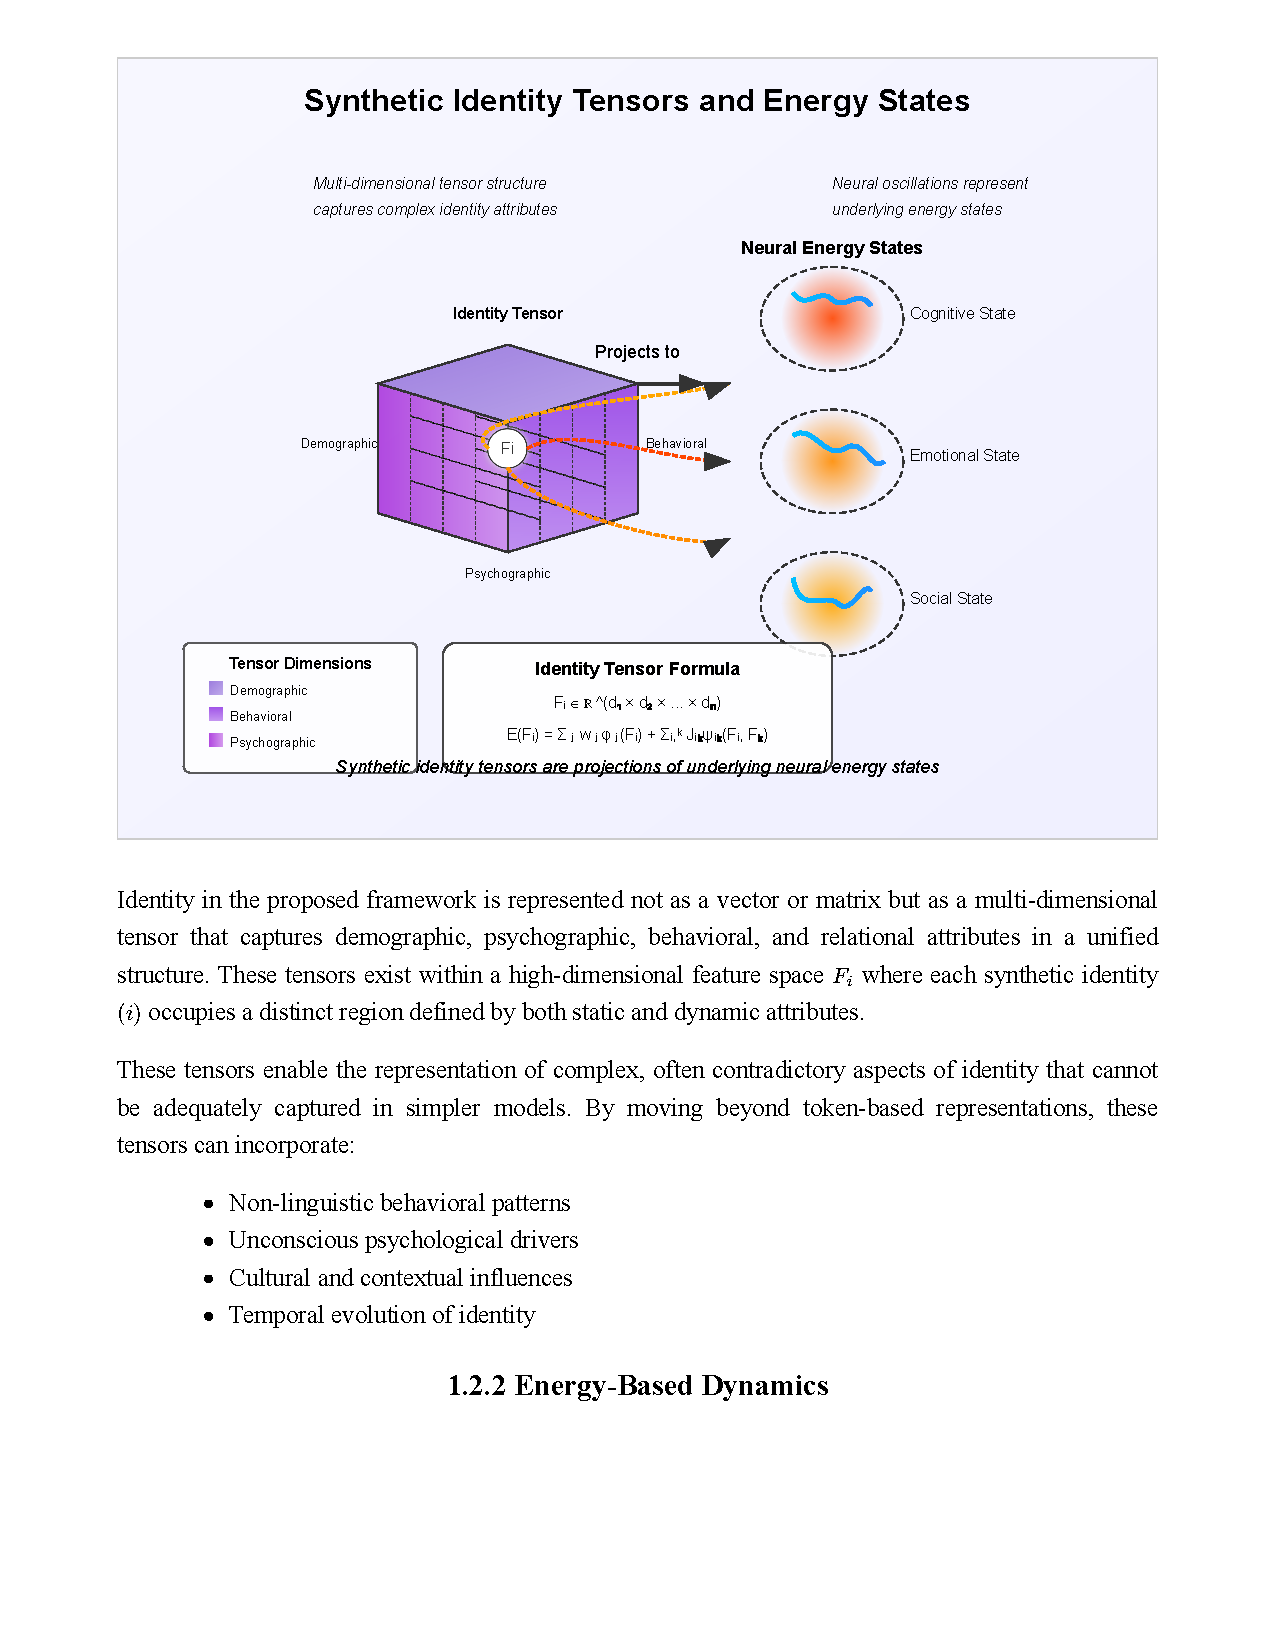
\includegraphics[width=0.8\textwidth]{synthetic_identity_tensors.pdf}
\caption{Synthetic Identity Tensors and Energy States}
\label{fig:identity_tensors}
\end{figure}

Identity in the proposed framework is represented not as a vector or matrix but as a multi-dimensional tensor that captures demographic, psychographic, behavioral, and relational attributes in a unified structure. These tensors exist within a high-dimensional feature space where each synthetic identity $F_i$ occupies a distinct region defined by both static and dynamic attributes.

These tensors enable the representation of complex, often contradictory aspects of identity that cannot be adequately captured in simpler models. By moving beyond token-based representations, these tensors can incorporate:

\begin{itemize}
\item Non-linguistic behavioral patterns
\item Unconscious psychological drivers
\item Cultural and contextual influences
\item Temporal evolution of identity
\end{itemize}

\subsubsection{Energy-Based Dynamics}

\begin{figure}[H]
\centering
% Figure showing ADPRS waveform patterns and social system energy landscape
% Should include: Multiple ADPRS waveforms with different A,D,P,R,S parameters
% Energy landscape with consensus, polarized, and fragmented states
% Transition paths and energy barriers
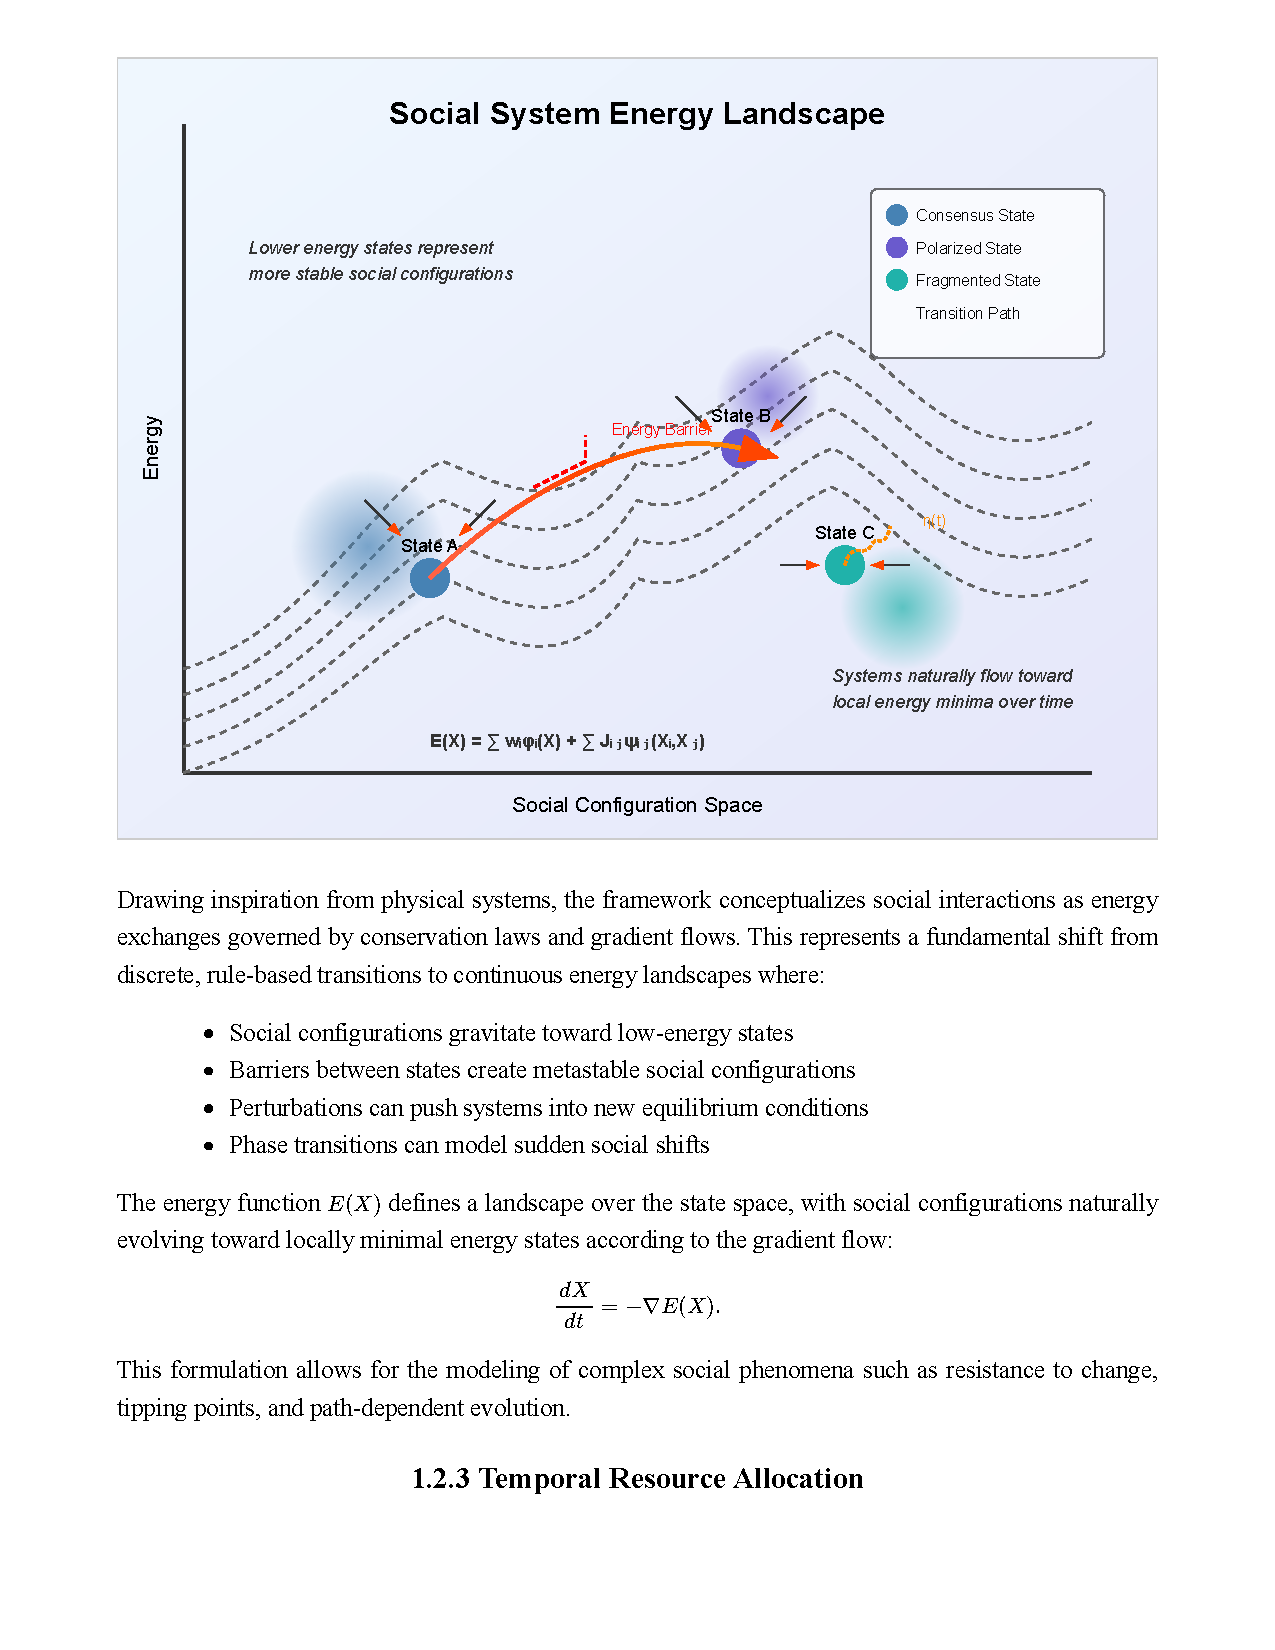
\includegraphics[width=0.8\textwidth]{adprs_energy_landscape.pdf}
\caption{ADPRS Waveform Patterns in Social Behavior and Social System Energy Landscape}
\label{fig:adprs_energy}
\end{figure}

Drawing inspiration from physical systems, the framework conceptualizes social interactions as energy exchanges governed by conservation laws and gradient flows. This represents a fundamental shift from discrete, rule-based transitions to continuous energy landscapes where:

\begin{itemize}
\item Social configurations gravitate toward low-energy states
\item Barriers between states create metastable social configurations
\item Perturbations can push systems into new equilibrium conditions
\item Phase transitions can model sudden social shifts
\end{itemize}

The energy function $E(X)$ defines a landscape over the state space, with social configurations naturally evolving toward locally minimal energy states according to the gradient flow:
\begin{equation}
\frac{dX}{dt} = -\nabla E(X).
\end{equation}

This formulation allows for the modeling of complex social phenomena such as resistance to change, tipping points, and path-dependent evolution.

\subsubsection{Temporal Resource Allocation}

Social behavior is fundamentally constrained by the finite nature of time and attention. The framework incorporates this constraint through a regulated allocation system $B(t)$ that governs how synthetic entities distribute their limited resources across potential activities.

This allocation follows optimization principles where:
\begin{itemize}
\item Each entity has a finite budget of time units
\item Activities have associated costs and benefits
\item Allocation decisions maximize utility subject to budget constraints
\item Temporal patterns emerge from consistent allocation preferences
\end{itemize}

The mathematical expression takes the form:
\begin{equation}
\max_{a_0,a_1,\ldots,a_T} \sum_{t=0}^T U(s_t, a_t) \text{ subject to } \sum_{t=0}^T B(s_t, a_t) \leq B_{\max}.
\end{equation}

\subsubsection{Synthetic Validation Mechanisms}

Unlike traditional models that lack internal consistency checks, the framework incorporates a multi-layered validation system that significantly reduces hallucinations and inconsistencies. This system operates through:

\begin{itemize}
\item Multiple synthetic validators with distinct expertise domains
\item Consistency checks against established identity attributes
\item Temporal feasibility verification
\item Behavioral pattern validation using waveform matching
\end{itemize}

The validation process is expressed as:
\begin{equation}
V(X_t \to X_{t+1}) = \prod_{i=1}^m \psi_i(X_t, X_{t+1}, C_i, H_t) \geq \theta_t,
\end{equation}
where $\psi_i$ represents individual validator functions and $\theta_t$ is a dynamic threshold that adapts based on the magnitude of the proposed state change.

\subsection{Transformative Implications}

This theoretical framework enables several transformative capabilities:

\begin{itemize}
\item \textbf{Universal Modeling}: The framework can model not only human social networks but also electrical networks, neural networks, and other complex systems with similar mathematical structures.
\item \textbf{De-hallucination}: By incorporating multi-layered validation mechanisms, the framework significantly reduces inconsistencies and impossibilities in synthetic simulations.
\item \textbf{Hyper-realism}: The tensor-based representation captures subtle aspects of identity and interaction that are missed by simpler models, leading to more realistic behavioral patterns.
\item \textbf{Temporal Coherence}: The structured approach to time prevents causality violations and ensures consistent behavioral evolution.
\end{itemize}

The integration of these principles creates a "strange loop" of validation where synthetic and simulated elements co-evolve within a shared temporal-social space, each reinforcing the other's development through continuous feedback mechanisms. This represents a fundamental advance in our ability to model, understand, and predict complex social phenomena.

\section{Modular Components and Synthetic Integration}

\subsection{Wavelets and Harmonic Analysis in Social Representations}

Traditional token-based representations in language models fail to capture the multi-scale, contextual nature of social phenomena. This framework introduces wavelet transforms and harmonic analysis as superior mathematical tools for representing social patterns across different scales and frequencies.

\subsubsection{From Tokens to Wavelets}

Instead of discrete tokens, social patterns are represented as continuous waveforms decomposed using wavelet transforms:
\begin{equation}
W_\psi f(s, u) = \int_{-\infty}^{\infty} f(t) \frac{1}{\sqrt{s}} \psi^*\left(\frac{t - u}{s}\right) dt,
\end{equation}
where:
\begin{itemize}
\item $f(t)$ is the social signal (behavior, communication, etc.)
\item $\psi$ is the mother wavelet function
\item $s$ is the scale parameter capturing phenomena at different resolutions
\item $u$ is the translation parameter situating the analysis in time
\end{itemize}

This wavelet representation offers several crucial advantages:
\begin{itemize}
\item Localization in both time and frequency domains
\item Multi-resolution analysis of social patterns
\item Efficient compression of social information
\item Robust handling of non-stationary behavior
\end{itemize}

\subsubsection{ADPRS Waveform Patterns}

Building on wavelet analysis, the framework introduces ADPRS (Asymptotic, Duration, Period, Recurrence, Spread) waveforms to model recurring behavioral patterns:
\begin{equation}
f_{\text{ADPRS}}(t) = A \cdot e^{-\lambda t} \cdot \sum_{k=0}^{\infty} D \cdot \text{rect}\left(\frac{t - kP}{D}\right).
\end{equation}

This formulation offers remarkable flexibility in modeling diverse social behaviors:
\begin{itemize}
\item \textbf{A (Asymptotic)}: Models long-term behavioral persistence
\item \textbf{D (Duration)}: Captures the sustained period of each behavior instance
\item \textbf{P (Period)}: Represents the interval between behavior instances
\item \textbf{R (Recurrence)}: Defined as $P/D$, measures frequency relative to duration
\item \textbf{S (Spread)}: Introduces stochastic variation in behavioral timing
\end{itemize}

These waveforms parallel the ADSR (Attack, Decay, Sustain, Release) envelopes used in audio synthesis, allowing social behaviors to be "composed" much like musical notes, with precise control over their temporal characteristics.

\subsection{Tensor-Augmented Markov Processes}

Traditional Markov processes, defined by transition matrices, cannot adequately capture the complex, context-dependent nature of social transitions. The framework extends this to tensor-augmented Markov processes that incorporate multi-dimensional contextual information.

\subsubsection{Higher-Order Tensor Transitions}

The transition dynamics are governed by a higher-order tensor operator:
\begin{equation}
\mathcal{T} \in \mathbb{R}^{n \times n \times d_1 \times d_2 \times \cdots \times d_k}.
\end{equation}

With transition probabilities determined by:
\begin{equation}
P(X_{t+1} = j \mid H_t) = \sum_{i_1,i_2,\ldots,i_k} \mathcal{T}_{X_t,j,i_1,i_2,\ldots,i_k} \cdot \phi_{i_1,i_2,\ldots,i_k}(H_t).
\end{equation}

This formulation allows transitions to depend on:
\begin{itemize}
\item Historical trajectories beyond just the current state
\item Environmental contexts and conditions
\item Multi-agent influences and group dynamics
\item Institutional and structural constraints
\end{itemize}

\subsubsection{Tensor Network Decompositions}

To manage computational complexity, the framework employs tensor network decompositions, particularly Matrix Product States (MPS) and Tensor Trains:
\begin{equation}
T_{i_1,i_2,\ldots,i_N} \approx \sum_{\alpha_1,\ldots,\alpha_{N-1}} A^1_{i_1,\alpha_1} A^2_{\alpha_1,i_2,\alpha_2} \cdots A^N_{\alpha_{N-1},i_N}.
\end{equation}

These decompositions offer:
\begin{itemize}
\item Exponential reduction in parameter space
\item Preservation of key correlations and dependencies
\item Efficient computation of transition probabilities
\item Scalability to larger social systems
\end{itemize}

\subsection{Clockchain and Synthetic Time}

A fundamental innovation in the framework is the "clockchain" mechanism that provides temporal anchoring and causal consistency throughout the synthetic social system.

\subsubsection{Directed Acyclic Graph of Time}

The clockchain is structured as a directed acyclic graph (DAG):
\begin{equation}
G_C = (V_C, E_C),
\end{equation}
where vertices represent temporal anchors and edges represent validated causal relationships between events. Each vertex contains a cryptographic hash linking it to predecessors:
\begin{equation}
h(v) = H(h(\text{pred}(v)), \text{state}(v), \text{timestamp}(v), \text{val}(v)).
\end{equation}

This structure ensures:
\begin{itemize}
\item Temporal consistency across the system
\item Immutable historical records
\item Verifiable causal relationships
\item Resistance to temporal paradoxes
\end{itemize}

\subsubsection{Synthetic Time as Source of Truth}

Unlike physical time, synthetic time can be manipulated, compressed, or expanded as needed while maintaining internal consistency. This flexible but structured approach to time serves as the principal source of truth in the system, regulating:
\begin{itemize}
\item Sequence validation (ensuring cause precedes effect)
\item Duration constraints (ensuring activities respect realistic time limits)
\item Synchronization across different subgraphs
\item Temporal references for validation operations
\end{itemize}

The synthetic time mechanism creates a consistent temporal framework without requiring external validation, enabling self-contained simulations that maintain temporal coherence.

\subsection{Synthetic Validator Networks}

To ensure consistency and reduce hallucinations, the framework incorporates networks of specialized synthetic validators.

\subsubsection{Validator Types and Functions}

The validator network includes several specialized types:
\begin{itemize}
\item \textbf{Identity Validators}: Ensure consistency with established identity tensors.
\item \textbf{Relationship Validators}: Verify compatibility with social network structure.
\item \textbf{Temporal Validators}: Check feasibility within time constraints.
\item \textbf{Pattern Validators}: Compare against established behavioral patterns.
\end{itemize}

Each validator $v_i$ has an associated credibility tensor $C_i \in \mathbb{R}^{d_c}$ and applies specialized validation functions:
\begin{equation}
\psi_i : S \times S \times \mathbb{R}^{d_c} \times H \to [0, 1].
\end{equation}

\subsubsection{Multi-Agent Consensus}

Validation requires consensus among multiple independent validators:
\begin{equation}
V(X_t \to X_{t+1}) = \prod_{i=1}^m \psi_i(X_t, X_{t+1}, C_i, H_t) \geq \theta_t.
\end{equation}

This multi-agent approach minimizes systematic biases in validation, enables specialized validation in different domains, creates redundancy to prevent single points of failure, and allows for graduated validation thresholds based on context.

\subsection{Meta-Tessera-CT Structure}

The overall organization of the system follows a "tessellated" structure that compartmentalizes different aspects of the social space.

\subsubsection{Tessera Definition and Construction}

Each tessera $\tau$ represents a subspace of the state space defined by constraint functions:
\begin{equation}
\tau = \{X \in S \mid g_1(X) = 0, g_2(X) = 0, \ldots, g_l(X) = 0\}.
\end{equation}

These tesserae can represent community boundaries, institutional contexts, cultural frameworks, or activity domains.

\subsubsection{Fiber Bundle Organization}

The Meta-Tessera-CT, denoted $M$, is organized as a fiber bundle:
\begin{equation}
M = \bigcup_{t \in T} \pi^{-1}(t),
\end{equation}
where $\pi : S \to T$ projects onto the temporal component and $\pi^{-1}(t)$ is the fiber over time point $t$. This structure enables efficient navigation of the system both temporally and socially, preserves relationships between different social contexts, allows for both top-down and bottom-up analysis, and supports multiple overlapping organizational principles.

\subsection{MAPEL Loop for Iterative Refinement}

The framework incorporates an iterative refinement mechanism called the MAPEL (Modeler, Adapter, Predictor, Evaluator, Learner) loop that continuously improves the system through feedback.

\subsubsection{Component Functions}

The MAPEL loop consists of:
\begin{itemize}
\item \textbf{Generator Function}: $G(\theta, X_t) = X_{t+1}$ (produces next states)
\item \textbf{Tester Function}: $T(X_t, X_{t+1}, c) \in [0, 1]$ (evaluates transitions)
\item \textbf{Helper Function}: $\theta_{t+1} = H(\theta_t, X_t, T(X_t, G(\theta_t, X_t), c))$ (updates parameters)
\end{itemize}

\subsubsection{Convergence Properties}

The loop converges when:
\begin{equation}
\lim_{t \to \infty} T(X_t, G(\theta_t, X_t), c) > \gamma.
\end{equation}

This iterative refinement adapts the system based on observed inconsistencies, gradually improves the realism of simulated behaviors, discovers latent patterns in social dynamics, and optimizes parameter values through experience.

\section{Mathematical Formalism and Implementation}

\subsection{Energy-Based Model Foundations}

\subsubsection{Energy Functional Definition}

The system defines an energy functional $E : S \to \mathbb{R}$ over the state space as:
\begin{equation}
E(X) = \sum_{i=1}^k w_i \phi_i(X) + \sum_{i,j} J_{ij} \psi_{ij}(X_i, X_j),
\end{equation}
where $\phi_i(X)$ represents local energy terms for individual entities, $\psi_{ij}(X_i, X_j)$ captures interaction energies between entities, and $w_i$ and $J_{ij}$ are weight parameters. This energy function incorporates social norms as energy penalties for norm violations, preferences as attractors in the energy landscape, relationships as coupling terms, and constraints as energy barriers between states.

\subsubsection{Gradient Flow Dynamics}

The evolution of the system follows gradient flow dynamics:
\begin{equation}
\frac{dX}{dt} = -\nabla E(X) + \eta(t),
\end{equation}
where $\eta(t)$ represents stochastic perturbations modeling the unpredictability of social behaviors. This formulation naturally produces convergence toward stable social configurations, resistance to small perturbations (social inertia), possible transitions between metastable states, and path-dependence in social evolution.

\subsubsection{Boltzmann Distribution and Statistical Mechanics}

At equilibrium, the probability of observing a particular state follows a Boltzmann distribution:
\begin{equation}
P(X) = \frac{1}{Z} e^{-\beta E(X)},
\end{equation}
where $\beta$ is an inverse temperature parameter controlling randomness and
\begin{equation}
Z = \sum_X e^{-\beta E(X)}
\end{equation}
is the partition function. This statistical mechanics framework enables calculation of expected system behaviors, characterization of phase transitions in social systems, analysis of entropy and information flow, and connection to maximum entropy principles.

\subsection{Wavelet and Fourier Transformations in the Model}

\subsubsection{Fourier Transform Application}

The Fourier transform extracts frequency domain representations of social signals:
\begin{equation}
\hat{f}(\omega) = \int_{-\infty}^{\infty} f(t)e^{-2\pi i\omega t} dt.
\end{equation}

Applied to social behavior, this transformation identifies periodic patterns, extracts dominant frequencies, enables filtering of noise, and supports compression of behavioral representations.

\subsubsection{Wavelet Transform Benefits}

The continuous wavelet transform applies wavelet analysis to social signals:
\begin{equation}
W_\psi f(s, u) = \int_{-\infty}^{\infty} f(t) \frac{1}{\sqrt{s}} \psi^*\left(\frac{t - u}{s}\right) dt.
\end{equation}

This approach offers localization in both time and frequency domains, multi-resolution analysis of social patterns, better handling of non-stationary behaviors, and preservation of transient phenomena.

\subsubsection{Application to Model Components}

These transformations are applied throughout the model:
\begin{itemize}
\item \textbf{Identity Tensor Transformation}: Identity tensors are projected into wavelet space to capture multi-scale attributes.
\item \textbf{Relationship Graph Transformation}: Social network edges are represented in frequency space to identify structural patterns.
\item \textbf{Behavioral Signal Processing}: ADPRS waveforms are processed using wavelet analysis to extract recurring patterns.
\item \textbf{Validation Pattern Matching}: Validators use wavelet coefficients for pattern matching and anomaly detection.
\end{itemize}

\subsection{Tensor Network Methods and Decompositions}

\subsubsection{Matrix Product State Representation}

The transition tensor is decomposed using Matrix Product States:
\begin{equation}
T_{i_1,i_2,\ldots,i_N} = \sum_{\alpha_1,\ldots,\alpha_{N-1}} A^1_{i_1,\alpha_1} A^2_{\alpha_1,i_2,\alpha_2} \cdots A^N_{\alpha_{N-1},i_N}.
\end{equation}

This decomposition reduces parameter count from exponential to linear in system size, preserves key correlations between neighboring components, enables efficient calculation of expectation values, and supports incremental updates.

\subsubsection{Tensor Renormalization Group}

For evolving systems, the framework employs Tensor Renormalization Group (TRG) methods:
\begin{equation}
T' = \mathcal{R}(T),
\end{equation}
where $\mathcal{R}$ is a renormalization operator that coarse-grains the system to capture essential dynamics, integrates out short-distance details, preserves long-range correlations, and enables analysis of scale-invariant properties.

\subsubsection{Practical Implementation}

The implementation uses several computational optimizations including sparse tensor representations, parallelized tensor contractions, truncated singular value decompositions to maintain manageable bond dimensions, and hierarchical tensor decompositions for multi-scale analysis.

\subsection{De-hallucination Mechanisms}

\subsubsection{Consistency Projection}

The de-hallucination process uses projection operations to maintain consistency:
\begin{equation}
X_{t+1} = (1 - \alpha_t)X_t + \alpha_t \Pi_{S_c}(X_t),
\end{equation}
where $\Pi_{S_c}(X)$ projects onto the consistent state subspace $\{X \in S \mid \Gamma(X) > \gamma_c\}$ and $\alpha_t \in [0, 1]$ controls the strength of the projection. This process gradually moves the system toward consistent configurations, preserves realistic transitions between states, adapts correction strength based on inconsistency magnitude, and maintains coherence while allowing innovation.

\subsubsection{Multi-layered Validation}

The validation process incorporates multiple independent checks:
\begin{equation}
\Gamma(X) = \exp\left(-\lambda \sum_{i=1}^k |C_i(X)|\right),
\end{equation}
where $C_i : S \to \mathbb{R}^{d_i}$ are constraint violation functions checking identity consistency, temporal feasibility, relationship compatibility, behavioral pattern coherence, and resource allocation validity.

\subsubsection{Temporal Anchoring}

The clockchain mechanism enforces causal consistency: events must respect temporal ordering constraints, cause must precede effect in all validated interactions, activities must fit within established time budgets, and temporal patterns must maintain consistency.

\subsection{Synthesizer-like Control Interface}

\subsubsection{Parameter Mapping}

The control interface maps intuitive parameters to underlying mathematical structures:
\begin{itemize}
\item Oscillator controls adjust identity tensor parameters
\item Envelope generators modify ADPRS behavioral waveforms
\item Filter controls adjust validation thresholds
\item Mixing controls determine interaction strengths
\end{itemize}

\subsubsection{Control Dimensions}

The interface provides several key control dimensions:
\begin{itemize}
\item \textbf{Intensity}: Controls the magnitude of behaviors and interactions
\item \textbf{Complexity}: Adjusts the dimensionality of identity tensors
\item \textbf{Coherence}: Modifies validation thresholds and consistency requirements
\item \textbf{Dynamics}: Controls temporal evolution rates and stochasticity
\end{itemize}

\subsubsection{Modulation and Parameter Automation}

The interface supports parameter modulation by low-frequency oscillators, automated parameter sequences following ADPRS patterns, cross-modulation between control parameters, and patch memory for storing and recalling configurations. This synthesizer-like approach enables the expression of complex social dynamics through intuitive controls, bridging the gap between mathematical formalism and creative exploration.

\subsection{Universal Applicability Beyond Human Social Systems}

\subsubsection{Electrical Networks}

For electrical networks:
\begin{itemize}
\item Nodes represent electrical components
\item Edges represent conductive pathways
\item Flow represents current
\item Potentials represent voltage
\item The energy function captures power dissipation
\end{itemize}

The same tensor-augmented Markov process can model current flow:
\begin{equation}
P(X_{t+1} = j \mid H_t) = \sum_{i_1,i_2,\ldots,i_k} T_{X_t,j,i_1,i_2,\ldots,i_k} \cdot \phi_{i_1,i_2,\ldots,i_k}(H_t).
\end{equation}

\subsubsection{Neural Networks}

For neural networks:
\begin{itemize}
\item Nodes represent neurons or neural populations
\item Edges represent synaptic connections
\item Flow represents activation patterns
\item ADPRS waveforms model neural firing patterns
\item The energy function captures network stability
\end{itemize}

\subsubsection{AI-to-AI Interactions}

For AI system interactions:
\begin{itemize}
\item Nodes represent AI agents with distinct capabilities
\item Edges represent communication channels
\item Flow represents information exchange
\item Validation mechanisms ensure coherent multi-agent behaviors
\item The energy function captures system optimization objectives
\end{itemize}

The universal applicability demonstrates the fundamental nature of the mathematical framework, which captures essential properties of complex networked systems regardless of their specific domain.

\subsection{Computational Complexity and Scalability}

\subsubsection{Complexity Analysis}

The time complexity for evaluating a single transition with $m$ validators in a state space of dimension $d$ is:
\begin{equation}
O(m \cdot d^2 \cdot \log(|V|)),
\end{equation}
and the space complexity for storing the system state and history is:
\begin{equation}
O(|S| + t \cdot |E|).
\end{equation}

\subsubsection{Optimization Strategies}

Several optimization strategies make the system computationally tractable:
\begin{itemize}
\item Tensor network decompositions reduce parameter count
\item Wavelet transformations enable efficient signal processing
\item Hierarchical validation focuses computational resources on likely inconsistencies
\item Temporal coarse-graining reduces historical state storage requirements
\item Parallelized validator operations distribute computational load
\end{itemize}

\subsubsection{Incremental Simulation}

The system supports incremental simulation where only actively observed regions are fully simulated, background regions evolve according to simplified models, validation intensity scales with interaction importance, and detailed simulation dynamically follows attention focus. These strategies enable practical implementation even for large-scale social systems with complex dynamics and rich temporal structure.

\section{Conclusion}

The Synthetic Social Graph Theorem presents a comprehensive mathematical framework for modeling social systems that transcends the limitations of token-based approaches. By integrating energy-based models, wavelet transformations, tensor networks, and synthetic validation mechanisms, the framework enables the creation of hyper-realistic social simulations with remarkable fidelity and internal consistency.

The shift from discrete tokens to continuous waveforms, from simple transitions to energy landscapes, and from unstructured time to clockchain validation represents a fundamental advance in our ability to model complex social phenomena. The synthesizer-like control interface bridges the gap between mathematical rigor and intuitive exploration, enabling both scientific investigation and creative expression.

The universal applicability of the framework to diverse systems—from human social networks to electrical circuits to AI agent collectives—demonstrates its fundamental nature. By capturing the essential mathematical structures underlying all complex networked systems, the framework provides a unified approach to modeling, understanding, and predicting their behavior.

Future work will focus on practical implementations, empirical validation, and extension to even more diverse application domains. As computational resources continue to advance, the full potential of this framework for creating truly hyper-realistic synthetic worlds will gradually be realized.

\end{document}
